\section{Evaluation}

% Authors: Keerthi Rapolu & Sreeja Katta

The evaluation asks whether earlier governance timing changes measurable system
outcomes. Each experiment targets one operational question: whether workload
intent can support accurate pre-execution forecasting, whether pre-billing
intervention prevents waste before launch, whether runtime governance remains
necessary after launch, whether intent-aware anomaly detection outperforms
utilization-only detection, and whether policy learning improves prevention over
time.

\subsection{Experimental Setup}

We evaluate PBCP on a controlled benchmark containing 500 workloads and 28{,}423
runs across six workload classes. The benchmark includes workload submissions,
historical run traces, cost records, runtime anomalies, and intervention stages
needed to evaluate pre-billing prevention, runtime governance, and policy
learning under one consistent workload-alignment setting.

\subsection{Exp 0: Can Simulation Predict Utilization Accurately?}

Exp~0 tests whether the simulator is accurate enough to support pre-billing
intervention. Figure~\ref{fig:exp0-calibration} and
Table~\ref{tab:exp0-results} show utilization MAE of 0.054 and cost rel-RMSE of
0.306. These errors are small enough for governance use even though they are not
perfect predictions of future execution. Operationally, the result matters
because pre-billing intervention only has value if simulation error is below the
threshold at which intervention becomes arbitrary. The remaining cost error is
also expected: duration varies at runtime, so a pre-execution model cannot fully
eliminate downstream uncertainty.

\begin{figure}[t]
\centering
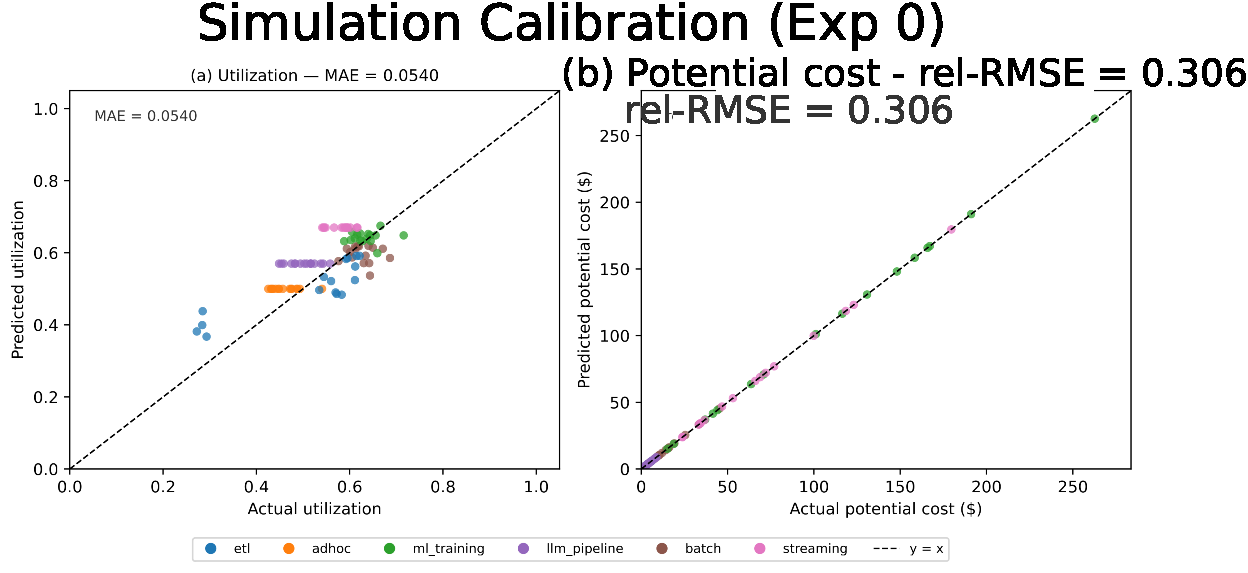
\includegraphics[width=\linewidth]{figures/exp0_calibration.pdf}
\caption{Simulation calibration for Exp~0. Predicted utilization tracks observed utilization closely, with utilization MAE of 0.054; the committed benchmark artifact also reports cost calibration on the same sample.}
\label{fig:exp0-calibration}
\end{figure}

\begin{table}[t]
\centering
\caption{Summary calibration results for Exp~0. The utilization error remains below the acceptance gate, and cost rel-RMSE stays within the tolerated pre-execution uncertainty range.}
\label{tab:exp0-results}
\begin{tabular}{lcc}
\toprule
Metric & Value & Gate \\
\midrule
Utilization MAE & 0.054 & $< 0.10$ \\
Cost rel-RMSE & 0.306 & $< 0.40$ \\
\bottomrule
\end{tabular}

\end{table}

\subsection{Exp 1: Can Pre-Provision Intervention Reduce Waste?}

Exp~1 evaluates whether pre-billing intervention prevents waste before resources
are launched. Figure~\ref{fig:exp1-preprovision} highlights the showcase case:
PBCP reduces a 20-node ETL request to 10 nodes before billing begins, preventing
\$15.36 with CPS of 0.500. The significance of this result is not the absolute
amount of prevented cost in one scenario, but the change in governance timing:
the waste path is altered before the cluster is ever provisioned. At the same
time, the broader benchmark reports relatively low system-wide CPS because most
requests are already near reasonable sizing. This behavior is desirable. A
pre-billing governance system should intervene strongly on high-divergence
requests without manufacturing unnecessary corrections on already aligned ones.

\begin{figure}[t]
\centering
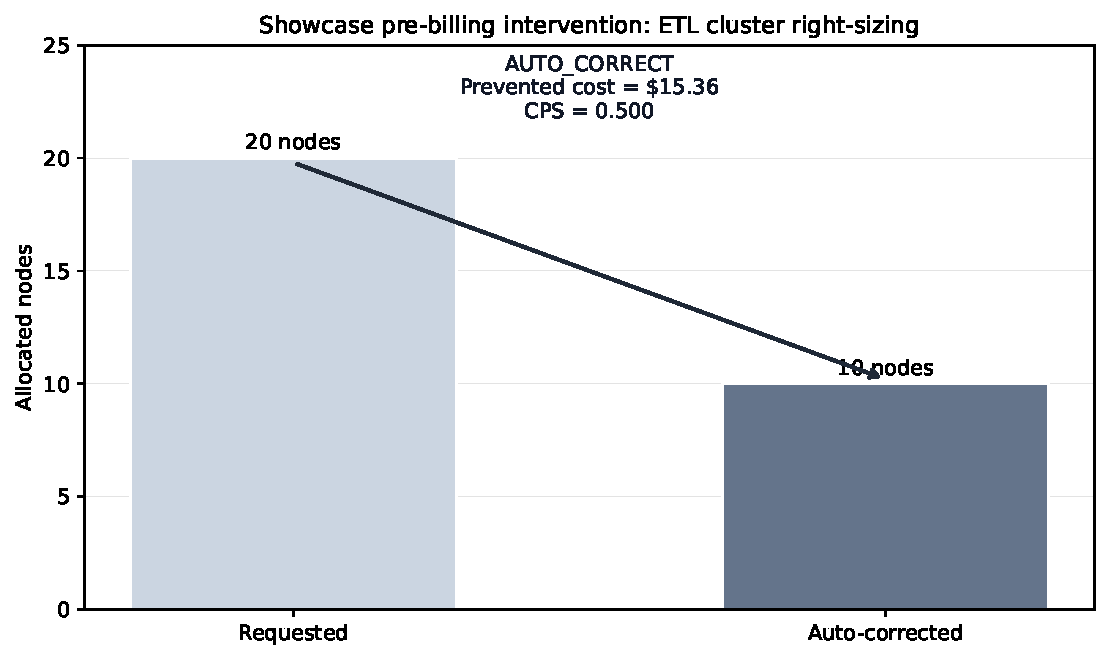
\includegraphics[width=0.78\linewidth]{figures/exp1_preprovision.pdf}
\caption{Showcase pre-provision intervention for a 20-node ETL request. PBCP auto-corrects the request to 10 nodes before billing begins, preventing \$15.36 with CPS of 0.500.}
\label{fig:exp1-preprovision}
\end{figure}

\subsection{Exp 2: Can Runtime Governance Catch Hidden Failures?}

Exp~2 evaluates whether runtime governance remains necessary after launch.
Figure~\ref{fig:exp2-runtime} and Table~\ref{tab:exp2-runtime} show that runtime
intervention captures failure modes that are only partially visible before
execution, including idle persistence, underutilized ETL execution, and runaway
ML training. The runaway scenario is especially important: the system prevents
\$97.92 with CPS of 0.667 by stopping additional cost accumulation after
divergence becomes operationally visible. These results suggest that runtime
governance is complementary to pre-billing intervention rather than redundant
with it; accurate pre-execution simulation reduces avoidable waste, but several
divergence patterns still emerge only after workload launch.

\begin{figure}[t]
\centering
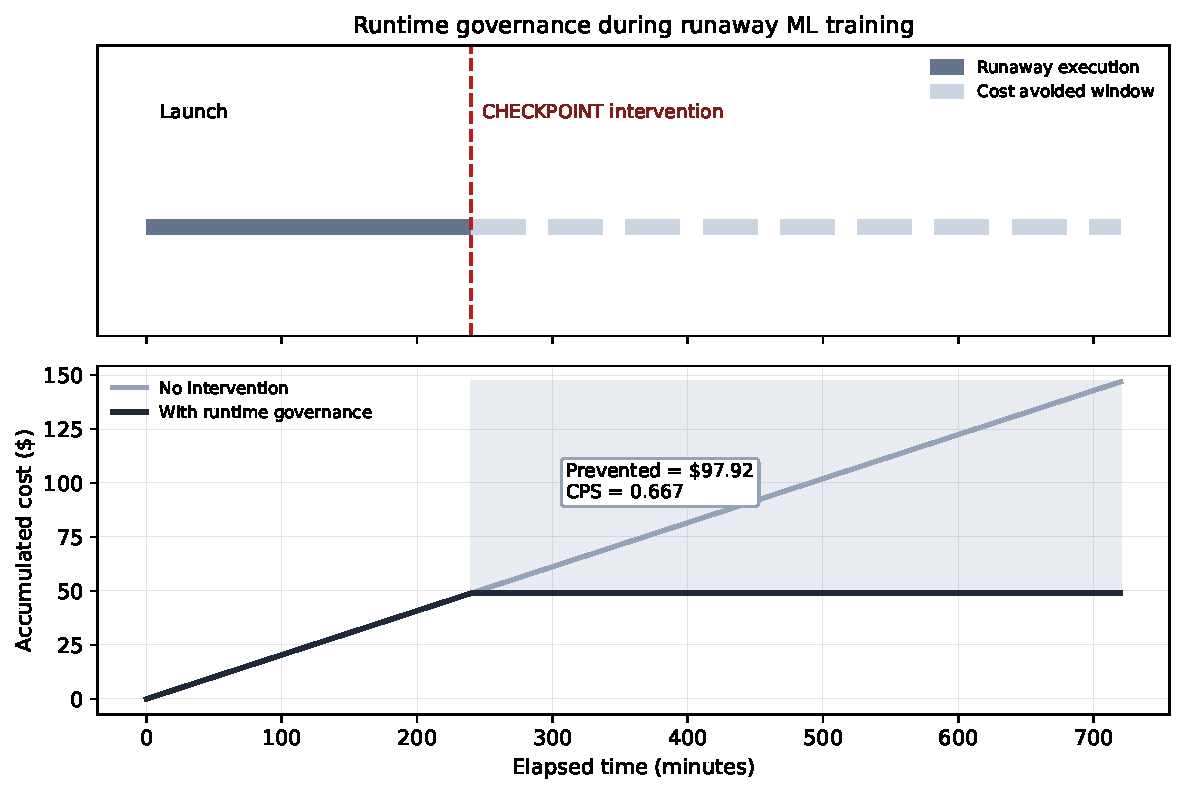
\includegraphics[width=0.9\linewidth]{figures/exp2_runtime_timeline.pdf}
\caption{Runtime governance intervention during a runaway ML training workload. The intervention checkpoints prolonged execution at the anomaly boundary, preventing \$97.92 of additional cost accumulation.}
\label{fig:exp2-runtime}
\end{figure}

\begin{table}[t]
\centering
\caption{Runtime intervention scenarios from Exp~2. These cases illustrate how runtime governance complements pre-billing control when hidden failures emerge only after launch.}
\label{tab:exp2-runtime}
\begin{tabular}{p{4.2cm}p{3.1cm}cc}
\toprule
Workload & Intervention & Prevented cost & CPS \\
\midrule
A Idle adhoc & SCALE\_DOWN, TERMINATE & $1.61$ & 0.932 \\
B Underutil ETL & SCALE\_DOWN & $21.50$ & 0.700 \\
C Runaway ML & CHECKPOINT & $97.92$ & 0.667 \\
\bottomrule
\end{tabular}

\end{table}

\subsection{Exp 3: Does IFS Outperform CPU-Threshold Detection?}

Exp~3 evaluates whether an intent-aware workload-alignment signal improves
anomaly detection relative to a utilization-only baseline. Figure~\ref{fig:exp3-detector}
and Table~\ref{tab:exp3-detector} show that the IFS-based detector improves F1
from 0.6054 to 0.7608 while substantially increasing recall. The operational
implication is that semantic alignment captures divergence missed by simple CPU
thresholding, particularly when anomalous behavior is not reducible to a single
utilization rule. At the same time, the subgroup comparison is mixed rather than
uniformly favorable, so the result should be interpreted as evidence that
intent-aware detection is stronger overall, not as proof that every workload
subgroup behaves identically.

\begin{figure}[t]
\centering
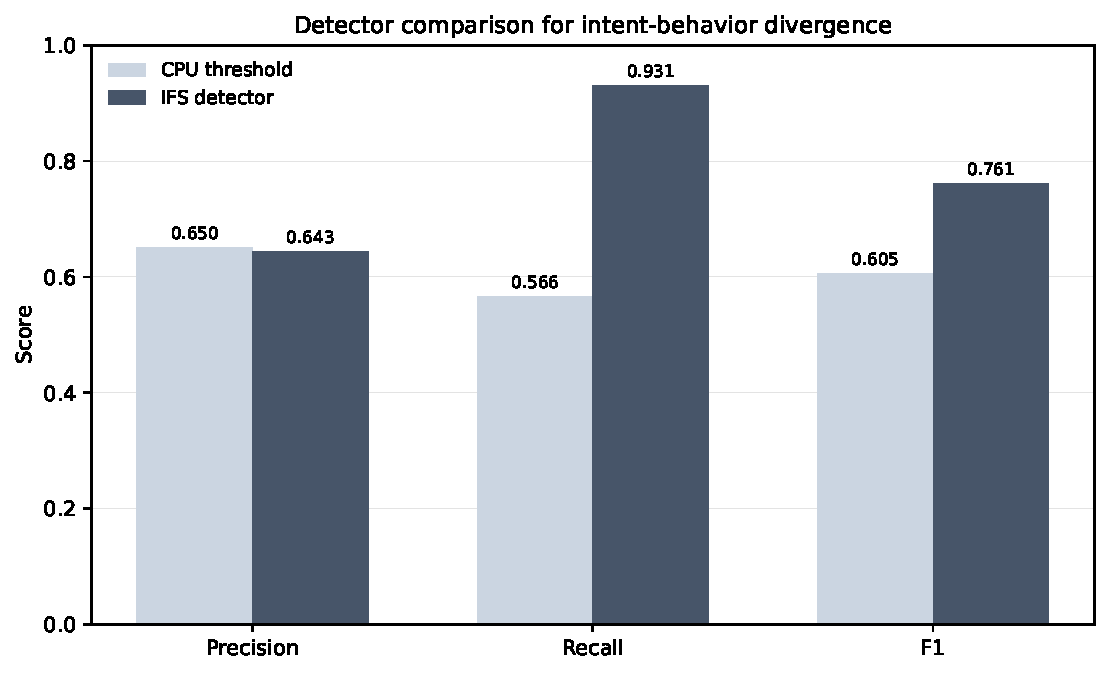
\includegraphics[width=0.8\linewidth]{figures/exp3_detector_comparison.pdf}
\caption{Detector comparison for Exp~3. The IFS-based detector improves overall detection quality relative to the CPU-threshold baseline on the committed benchmark outputs.}
\label{fig:exp3-detector}
\end{figure}

\begin{table}[t]
\centering
\caption{Detector metrics for Exp~3. Values are taken directly from the recorded IBD evaluation outputs.}
\label{tab:exp3-detector}
\begin{tabular}{lccc}
\toprule
Detector & Precision & Recall & F1 \\
\midrule
CPU threshold & 0.6502 & 0.5663 & 0.6054 \\
IFS detector & 0.6434 & 0.9306 & 0.7608 \\
\bottomrule
\end{tabular}

\end{table}

% Authors: Keerthi Rapolu & Sreeja Katta

The F1 improvement from 0.605 to 0.761 is driven primarily by recall. The
IFS-based detector captures anomalous workloads that the CPU-threshold baseline
classifies as normal because their utilization does not breach the detection
boundary. This pattern is consistent with the design intent of IFS: a workload
that finishes early and idles, consumes fewer resources than requested, or
executes a materially different computation than its description implies can
remain below the utilization alert threshold while still producing measurable
intent-behavior divergence.

The mismatch-subgroup result adds an important qualification. Among workloads
flagged as type-mismatched by intent inference, anomaly rates are higher and
mean IFS is lower than in the non-mismatch group, consistent with the hypothesis
that declared-to-inferred type divergence predicts runtime divergence. However,
the anomaly rate difference across subgroups is not large enough for type
mismatch alone to serve as a reliable detection signal. The subgroup result
supports IFS as a composite detector rather than suggesting that any single
structural feature is sufficient.

The precision tradeoff is also worth stating directly. IFS precision on this
benchmark is lower than the CPU-threshold baseline, meaning intent-aware
detection produces more false positives per true positive. This is a consequence
of IFS operating at broader sensitivity: it flags misaligned workloads earlier
and more broadly than a utilization gate would. The threshold sweep shows that an
operator can recover precision by raising $\theta_{\mathrm{ifs}}$ at the cost of
recall, which provides a practical tuning handle once deployed against a
production workload population.


\subsection{Exp 5: What Is Overall System Effectiveness?}

Exp~5 provides a system-level roll-up using CPS, ESR, and IFS together. This
combination matters because prevention quality, execution safety, and workload
alignment answer different questions. CPS alone can overstate success if a
system avoids cost by over-blocking workloads, while ESR alone cannot indicate
whether meaningful waste was prevented. IFS adds diagnostic structure by showing
whether low-cost outcomes are associated with aligned workload behavior rather
than with arbitrary restriction. In the recorded benchmark, PBCP reaches Valid
CPS of 0.5585 with ESR of 0.9809, indicating that prevention remains high even
after discounting unsuccessful or overly aggressive intervention behavior. Taken
together, the roll-up suggests that the system can improve economic prevention
while preserving useful execution and maintaining meaningful workload
alignment.

\subsection{Exp 6: Does Policy Learning Improve Over Time?}

Exp~6 evaluates whether policy learning improves governance quality over time.
Figure~\ref{fig:exp6-convergence} and Table~\ref{tab:exp6-ablation} show that
Full PBCP reaches peak CPS of 0.733, whereas the No Phase 3 baseline peaks at
0.013. This 56$\times$ separation is the strongest evidence that the learning
loop changes system behavior rather than merely documenting it. The ablation
comparison also clarifies what is being learned: static policy-only control
contributes little in this setting, and embedding-only retrieval is useful but
insufficient by itself. Governance quality improves most when workload
alignment, intervention policy, and feedback are integrated into one loop rather
than deployed as isolated components.

\begin{figure}[t]
\centering
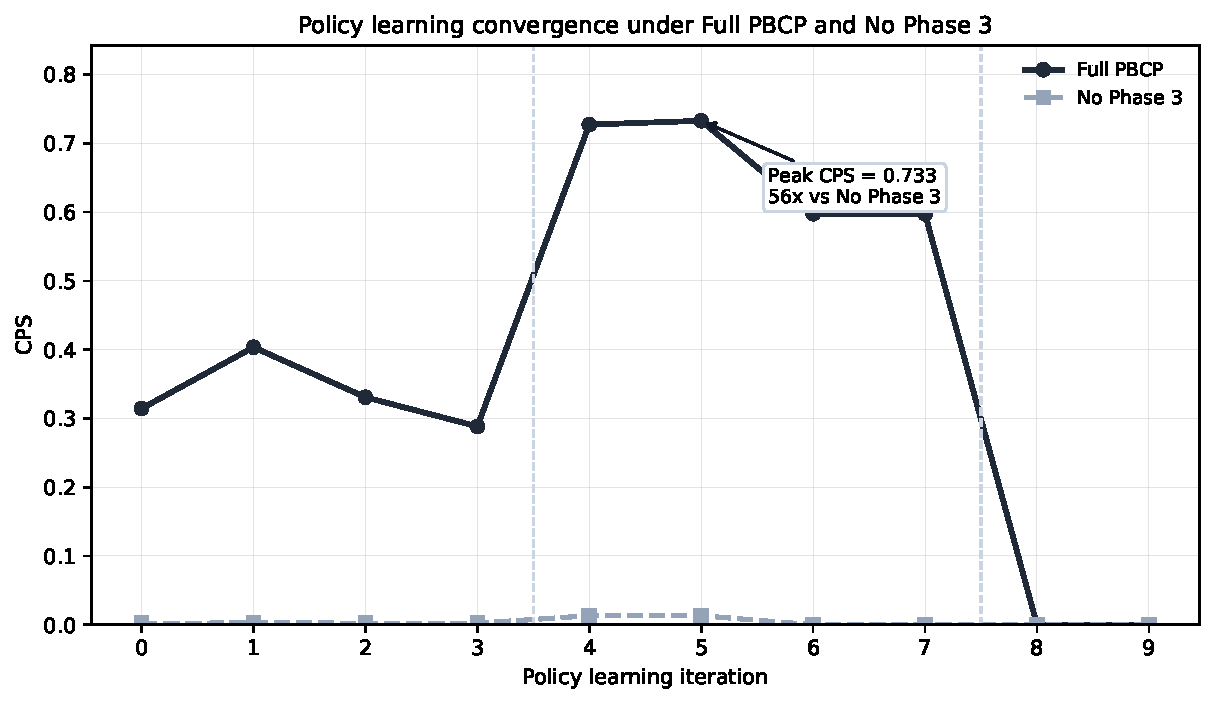
\includegraphics[width=\linewidth]{figures/exp6_convergence.pdf}
\caption{Policy-learning convergence in Exp~6. Full PBCP reaches peak CPS of 0.733, compared with 0.013 for the No Phase 3 baseline, demonstrating a 56$\times$ improvement at peak.}
\label{fig:exp6-convergence}
\end{figure}

\begin{table}[t]
\centering
\caption{Available Exp~6 ablations from the committed benchmark outputs. Peak CPS is reported for each variant without relabeling unsupported baselines.}
\label{tab:exp6-ablation}
\begin{tabular}{lcc}
\toprule
Variant & Peak CPS & Peak generation \\
\midrule
Full PBCP & 0.733 & 5 \\
No Phase 3 & 0.013 & 4 \\
Policy-only & 0.000 & 0 \\
Embedding-only & 0.109 & 2 \\
\bottomrule
\end{tabular}

\end{table}
